\section{Introduction}

In this lab, we tested the effects of friction on a cart with a bottom comprised of various materials sliding down a slope.

\section{Procedure}

The track that the carts were slid down was set up by using two large frames and propping up the track between them.
The track itself was braced against the ground to prevent it from wobbling.

The track's angle and the cart's mass was adjusted until the cart would slide down in a reasonable amount of time (enough to take some readings).
This was done by testing.
The resulting angle and masses were measured.

The motion sensor was affixed to the top of the track, and pointed down parallel to the track.

\begin{figure}[h]

\begin{center}
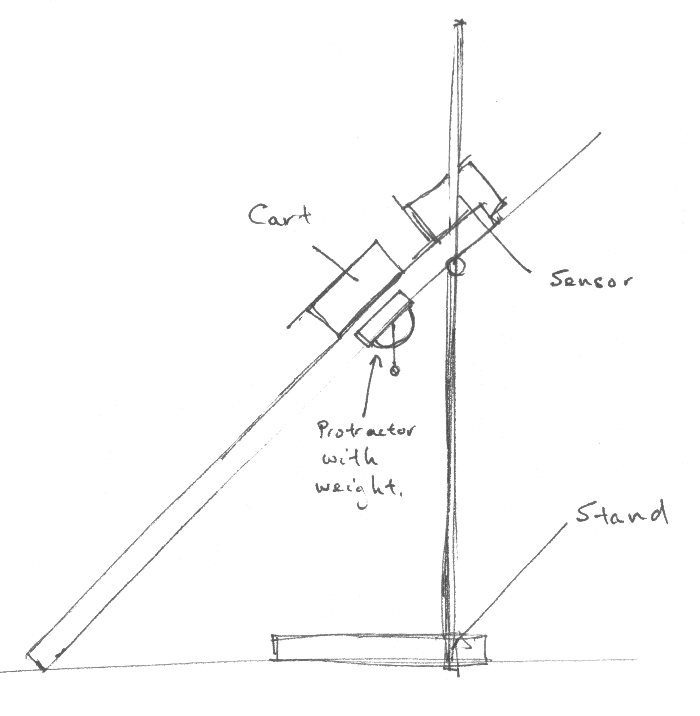
\includegraphics[scale=0.3]{content/fig1}
\end{center}

\caption{The setup of this lab.}

\end{figure}

Four carts were prepared, each with a different base, in order to get different coefficients of friction.
The carts were slid down the inclined track, and their various accelerations were recorded by the motion sensor.

To test static friction, the carts were placed motionless on the track, and the track was lifted slowly at one end until the cart began sliding.
The angle at which it began sliding was recorded.

\section{Results and Discussion}

\subsection{Questions}

\begin{enumerate}

\item Is the acceleration of the motion cart constant? Why or why not?

It can be said to be constant in all the recorded tests, as the variation in each measurement is generally lower than the standard deviation for that set of data.

\item Does the friction force depend on the mass of the cart? How about the friction coefficient, \begin{math}\mu\end{math}?

The friction force, in theory, should depend on the mass of the cart, since the mass of the cart will affect the magnitude of the normal force between the cart and track.
However, we were not able to effectively run tests with many different masses, so we have no emperical confirmation of that theory.

The friction coefficient definitely affects the friction force --- the different materials we tested resulted in various different accelerations, with cork being the highest and marble being the lowest.
The tests bore out results consistent with the idea that a larger coefficient would result in larger frictional forces.

\item What is the relationship between the angle the cart starts to slide at and the coefficient of friction?

As the coefficient gets larger, the angle needs to be steeper before the cart will start moving.
Our highest value was with the cork cart, which nearly went up to 40 degrees before starting to slide.

\item What is the Newton's third force pair to friction? Draw a free-body diagram.

Third force pairs must always be opposed to each other, the pair for friction must be in the direction of motion.

\begin{figure}[h]

\begin{center}
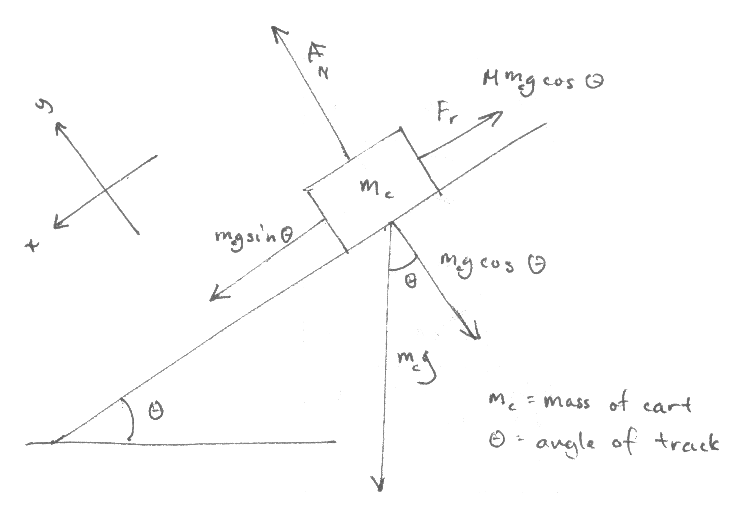
\includegraphics[scale=0.3]{content/fig2}
\end{center}

\caption{Free-body diagram for the system.}

\end{figure}

\item Does the friction force depend on contact surface area? Why or why not? How can you test this?

It does not, in theory, depend on contact surface area, as the equation is purely related to the magnitude of the normal force.
We could possibly test this by using carts with variously different sized contact surfaces.
Should they not exhibit any significant change in acceleration, all else being equal, we would be able to conclude that the surface area has little or no bearing on the friction force.

\end{enumerate}

\subsection{Error Analysis}

The main sources of error are hard to discern for this experiment.
The first and foremost issue comes from the readings themselves --- in some cases, the standard deviation was larger than the actual readings recorded, making figuring out a reasonable range for the readings
rather difficult at best.
The readings were all clipped off at the start and end so that the not-yet-accelerating parts before the cart was released and when it hit the ground were not taken into account,
but it is possible that other data may have been clipped off in the process, as well.

\section{Conclusion}

The frictional coefficients of the various materials vary widely, and have a noticeable and easily measurable bearing on the effects of the frictional force.

